\indent\textbf{Цель работы:} изучить спектры сигналов различной формы и влияние параметров сигнала на вид соответствующих спектров; проверить справедливость соотношений неопределённостей; познакомиться с работой спектральных фильтров на примере RC-цепочки.\\\indent
\textbf{Оборудование:} генератор сигналов произвольной формы, цифровой осциллограф с функцией быстрого преобразования Фурье или цифровой USB-осциллограф, подключённый к персональному компьютеру.\\
\subsection*{Исследование спектра периодической последовательности прямоугольных импульсов и проверка соотношений неопределенности}

\begin{figure}[h!]
    \centering
    \begin{subfigure}{.6\linewidth}
        \centering
        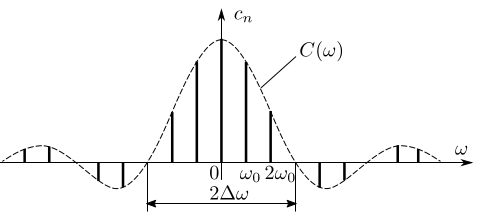
\includegraphics[width=8cm]{images/spectr.png}
    \end{subfigure}
    \hfill
    \begin{subfigure}{.39\linewidth}
        \centering
        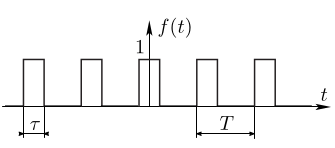
\includegraphics[width=6cm]{images/periodic_signals.png}
    \end{subfigure}
    \caption{Периодическая последовательность импульсов и её спектр}
\end{figure}
Найдем спектр периодической последовательности прямоугольных импульсов длительности $\tau$ и периодом следования импульсов $T > \tau$:
\begin{equation}
    c_n = \frac{1}{T}\int_{-\tau / 2}^{\tau / 2} e^{-in\omega_0t}dt = \frac{\tau}{T}\cdot\frac{\sin({\pi n \tau / T)}}{n\omega_0 \tau / 2} = \frac{\sin(\pi n\tau /T) }{\pi n}
\end{equation}
\indent Тогда представленные ниже фотографии лекго объяснить. При увеличении частоты повторения синус растет, а с ним и амплитуда гармоник. При этом кол-во гармоник в полуширине уменьшается т.к частота повторения растет. Если же увеличивать длительность импульса, то амплитуда гармоник растет, а ширина $\Delta \omega$ уменьшается.
\newpage
\begin{figure}[h!]
    \centering
    \begin{subfigure}[b]{0.3\linewidth}
        \centering
        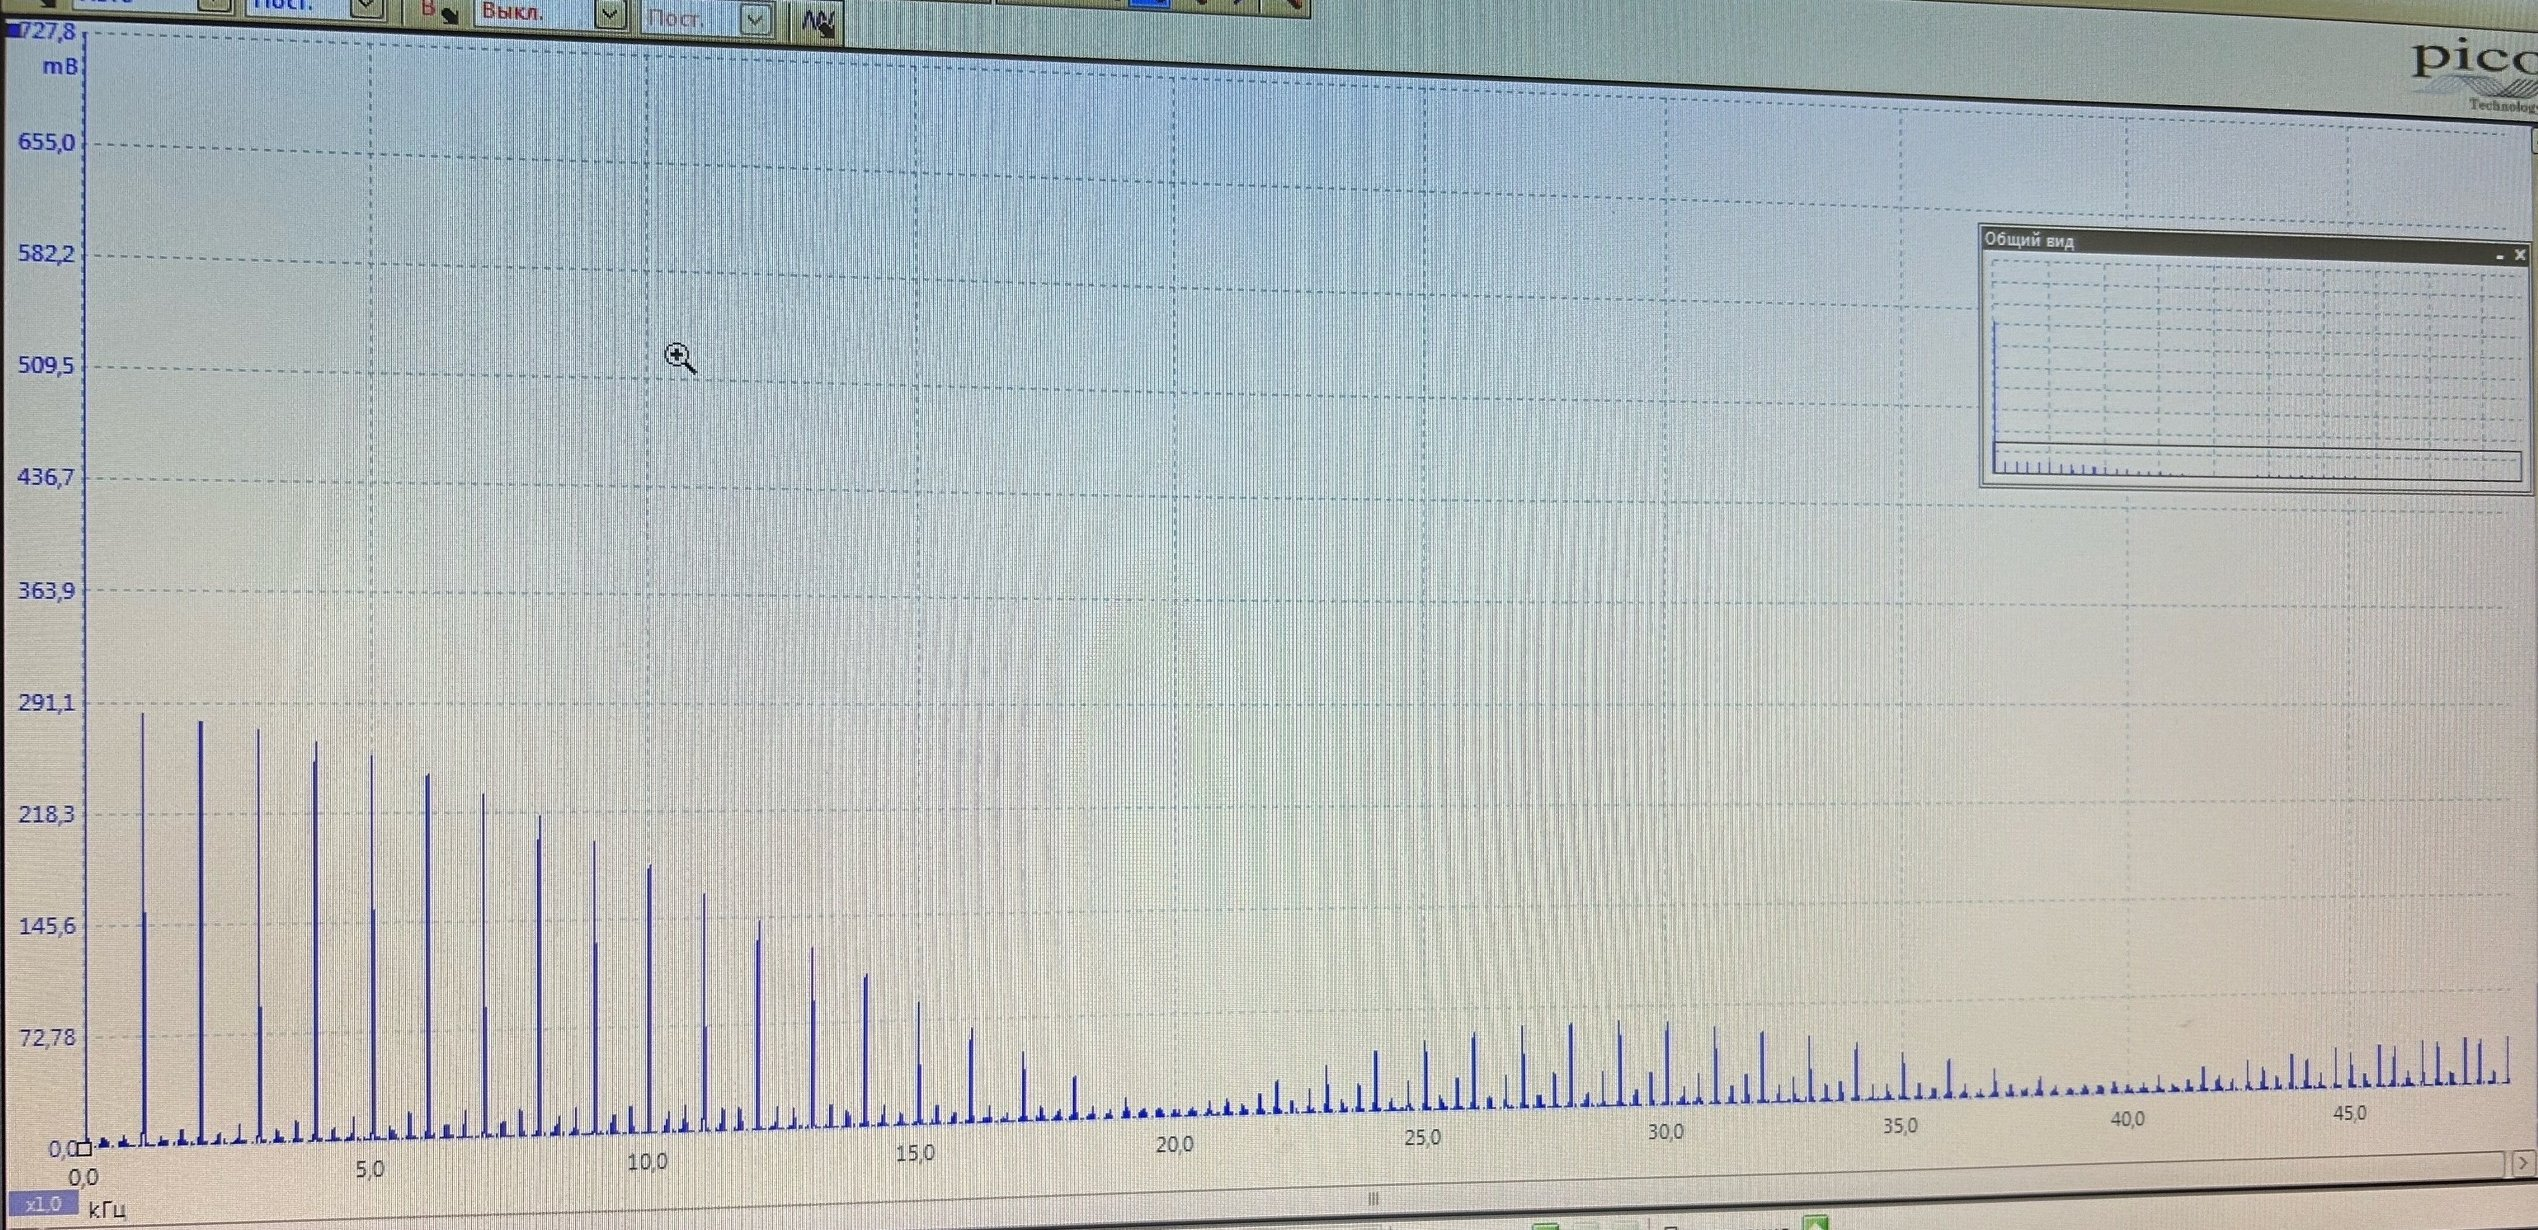
\includegraphics[width=6cm]{./images/nu_1_t_50.jpg}
        \caption{$\nu_{повт} = 1$кГц; $\tau = 50$ мкс}
    \end{subfigure}
    \hfill
    \begin{subfigure}[b]{0.3\linewidth}
        \centering
        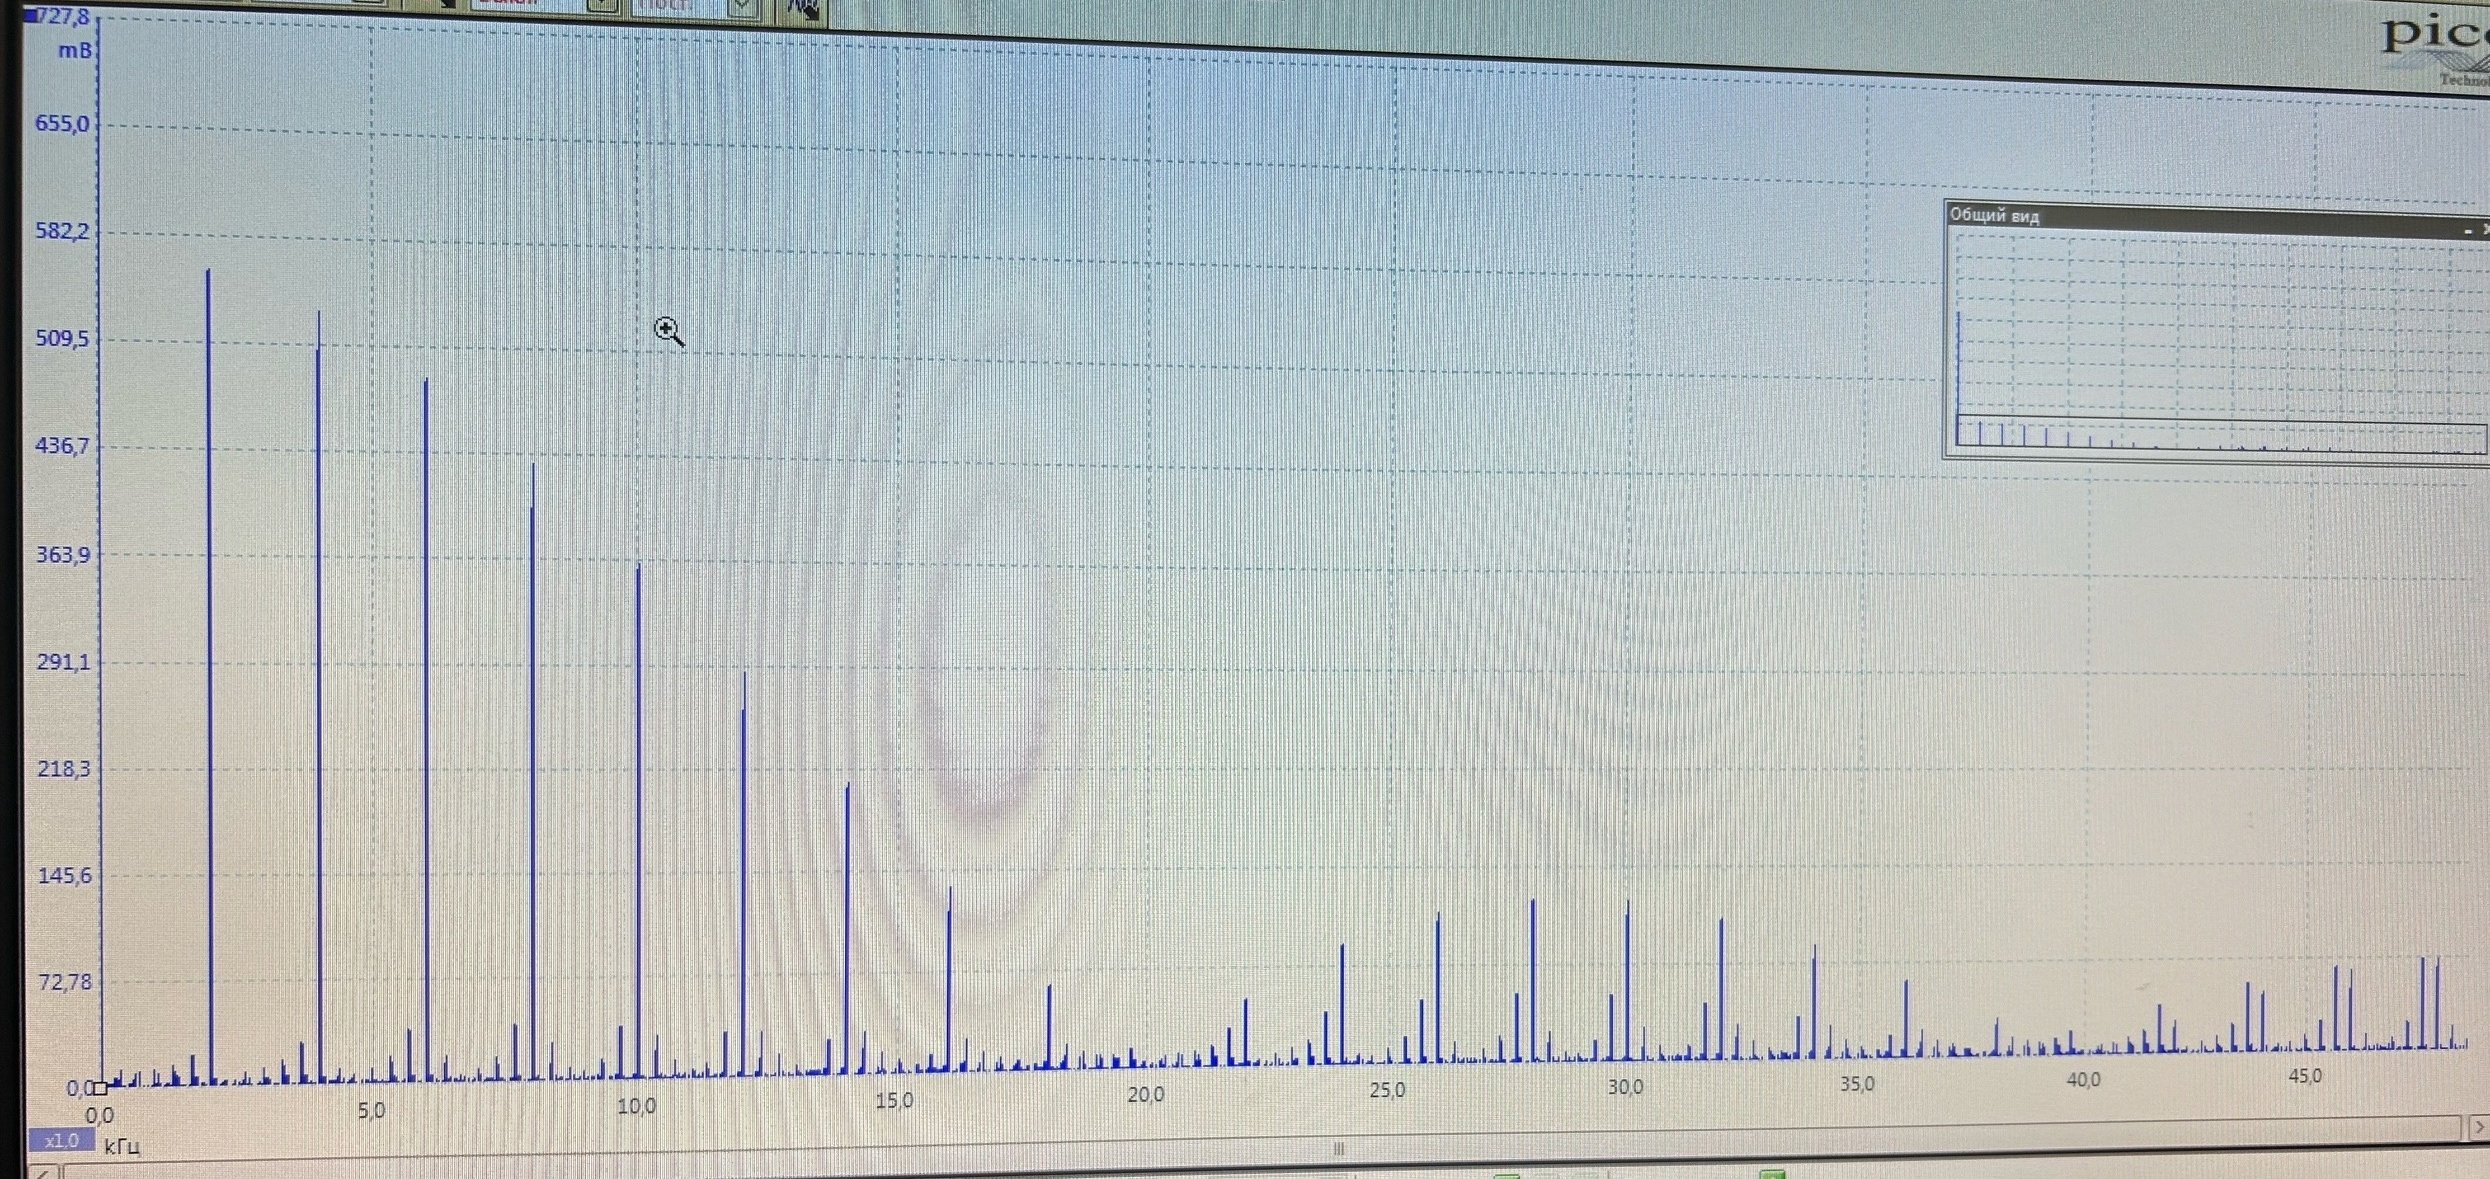
\includegraphics[width=6cm]{./images/nu_2_t_50.jpg}
        \caption{$\nu_{повт} = 2$кГц; $\tau = 50$ мкс}
    \end{subfigure}
    \hfill
    \begin{subfigure}{0.3\linewidth}
        \centering
        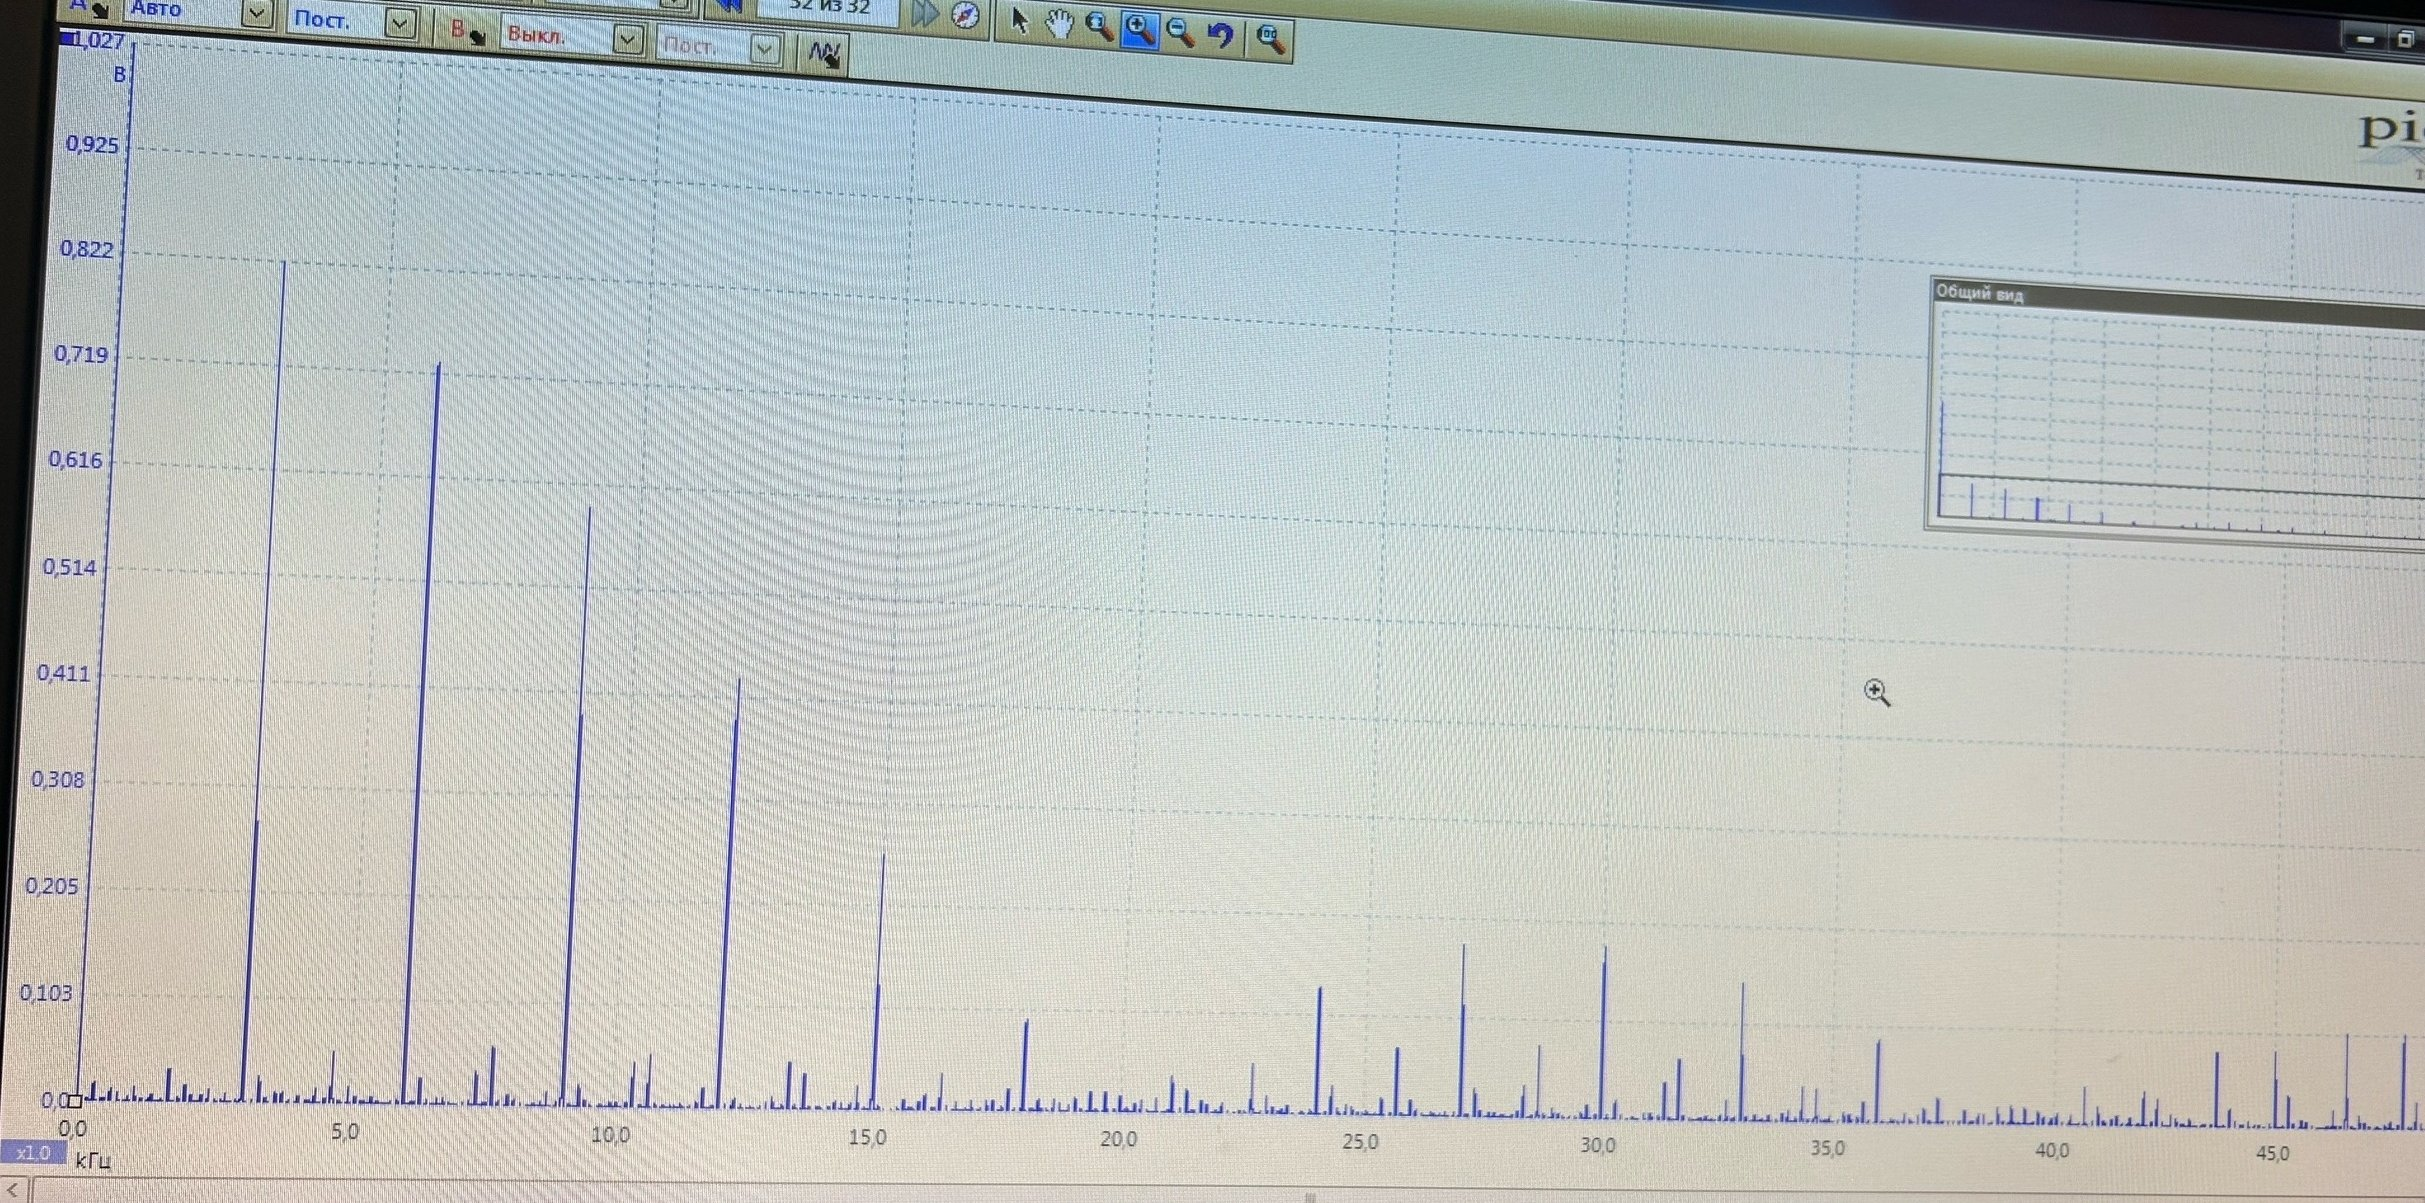
\includegraphics[width=6cm]{./images/nu_3_t_50.jpg}
        \caption{$\nu_{повт} = 3$кГц; $\tau = 50$ мкс}
    \end{subfigure}
    \vfill
    \begin{subfigure}{0.35\linewidth}
        \centering
        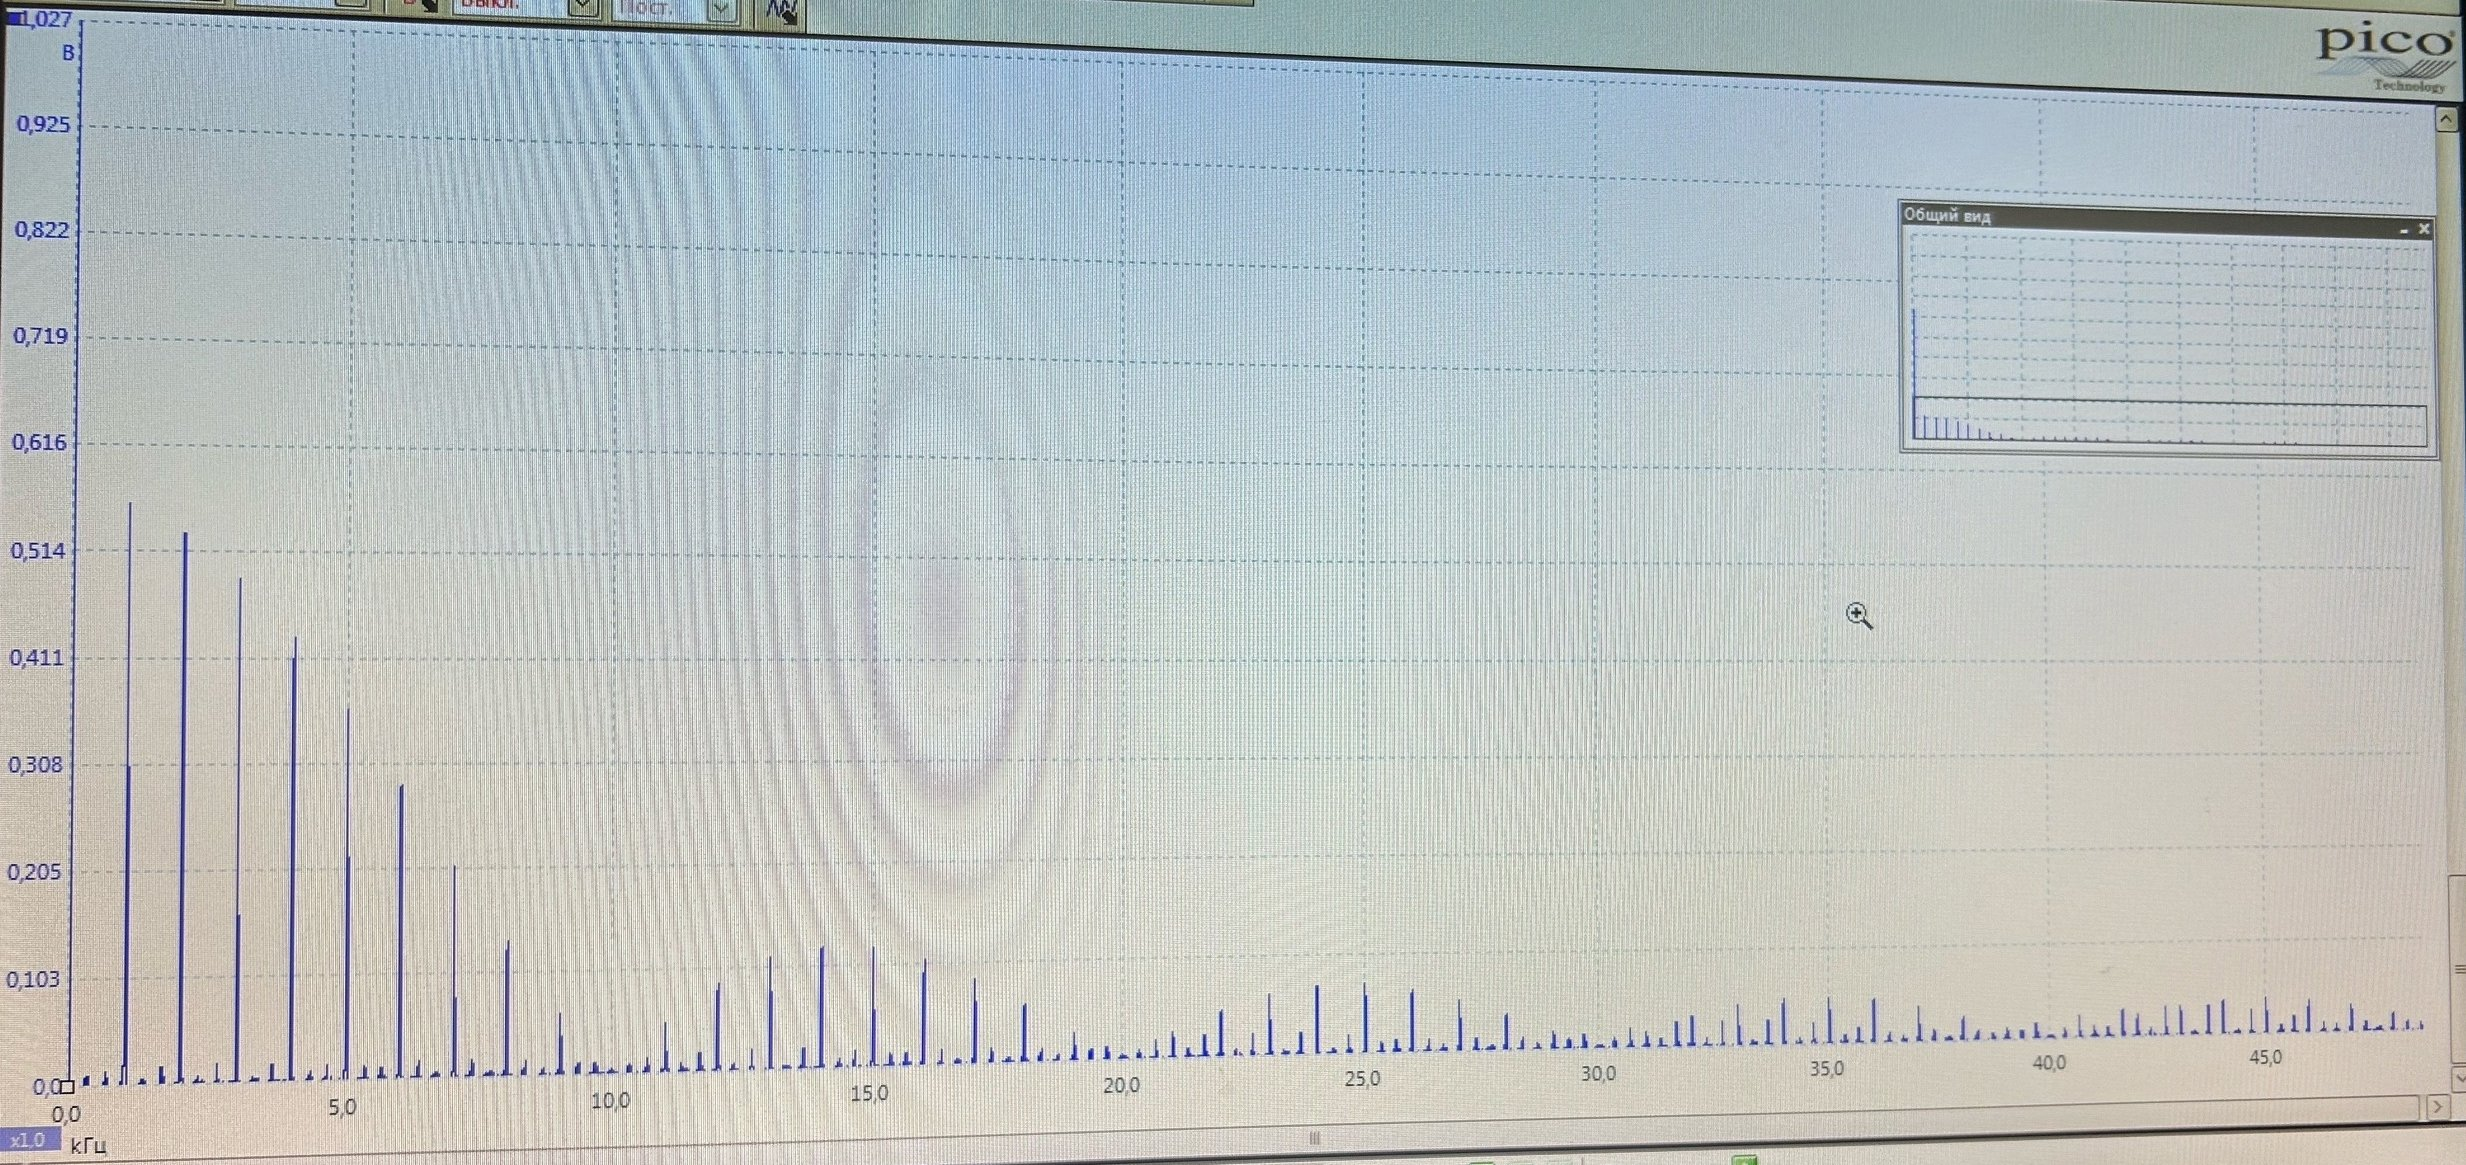
\includegraphics[width=6cm]{./images/nu_1_t_100.jpg}
        \caption{$\nu_{повт} = 1$кГц; $\tau = 100$ мкс}
    \end{subfigure}
    \begin{subfigure}{0.35\linewidth}
        \centering
        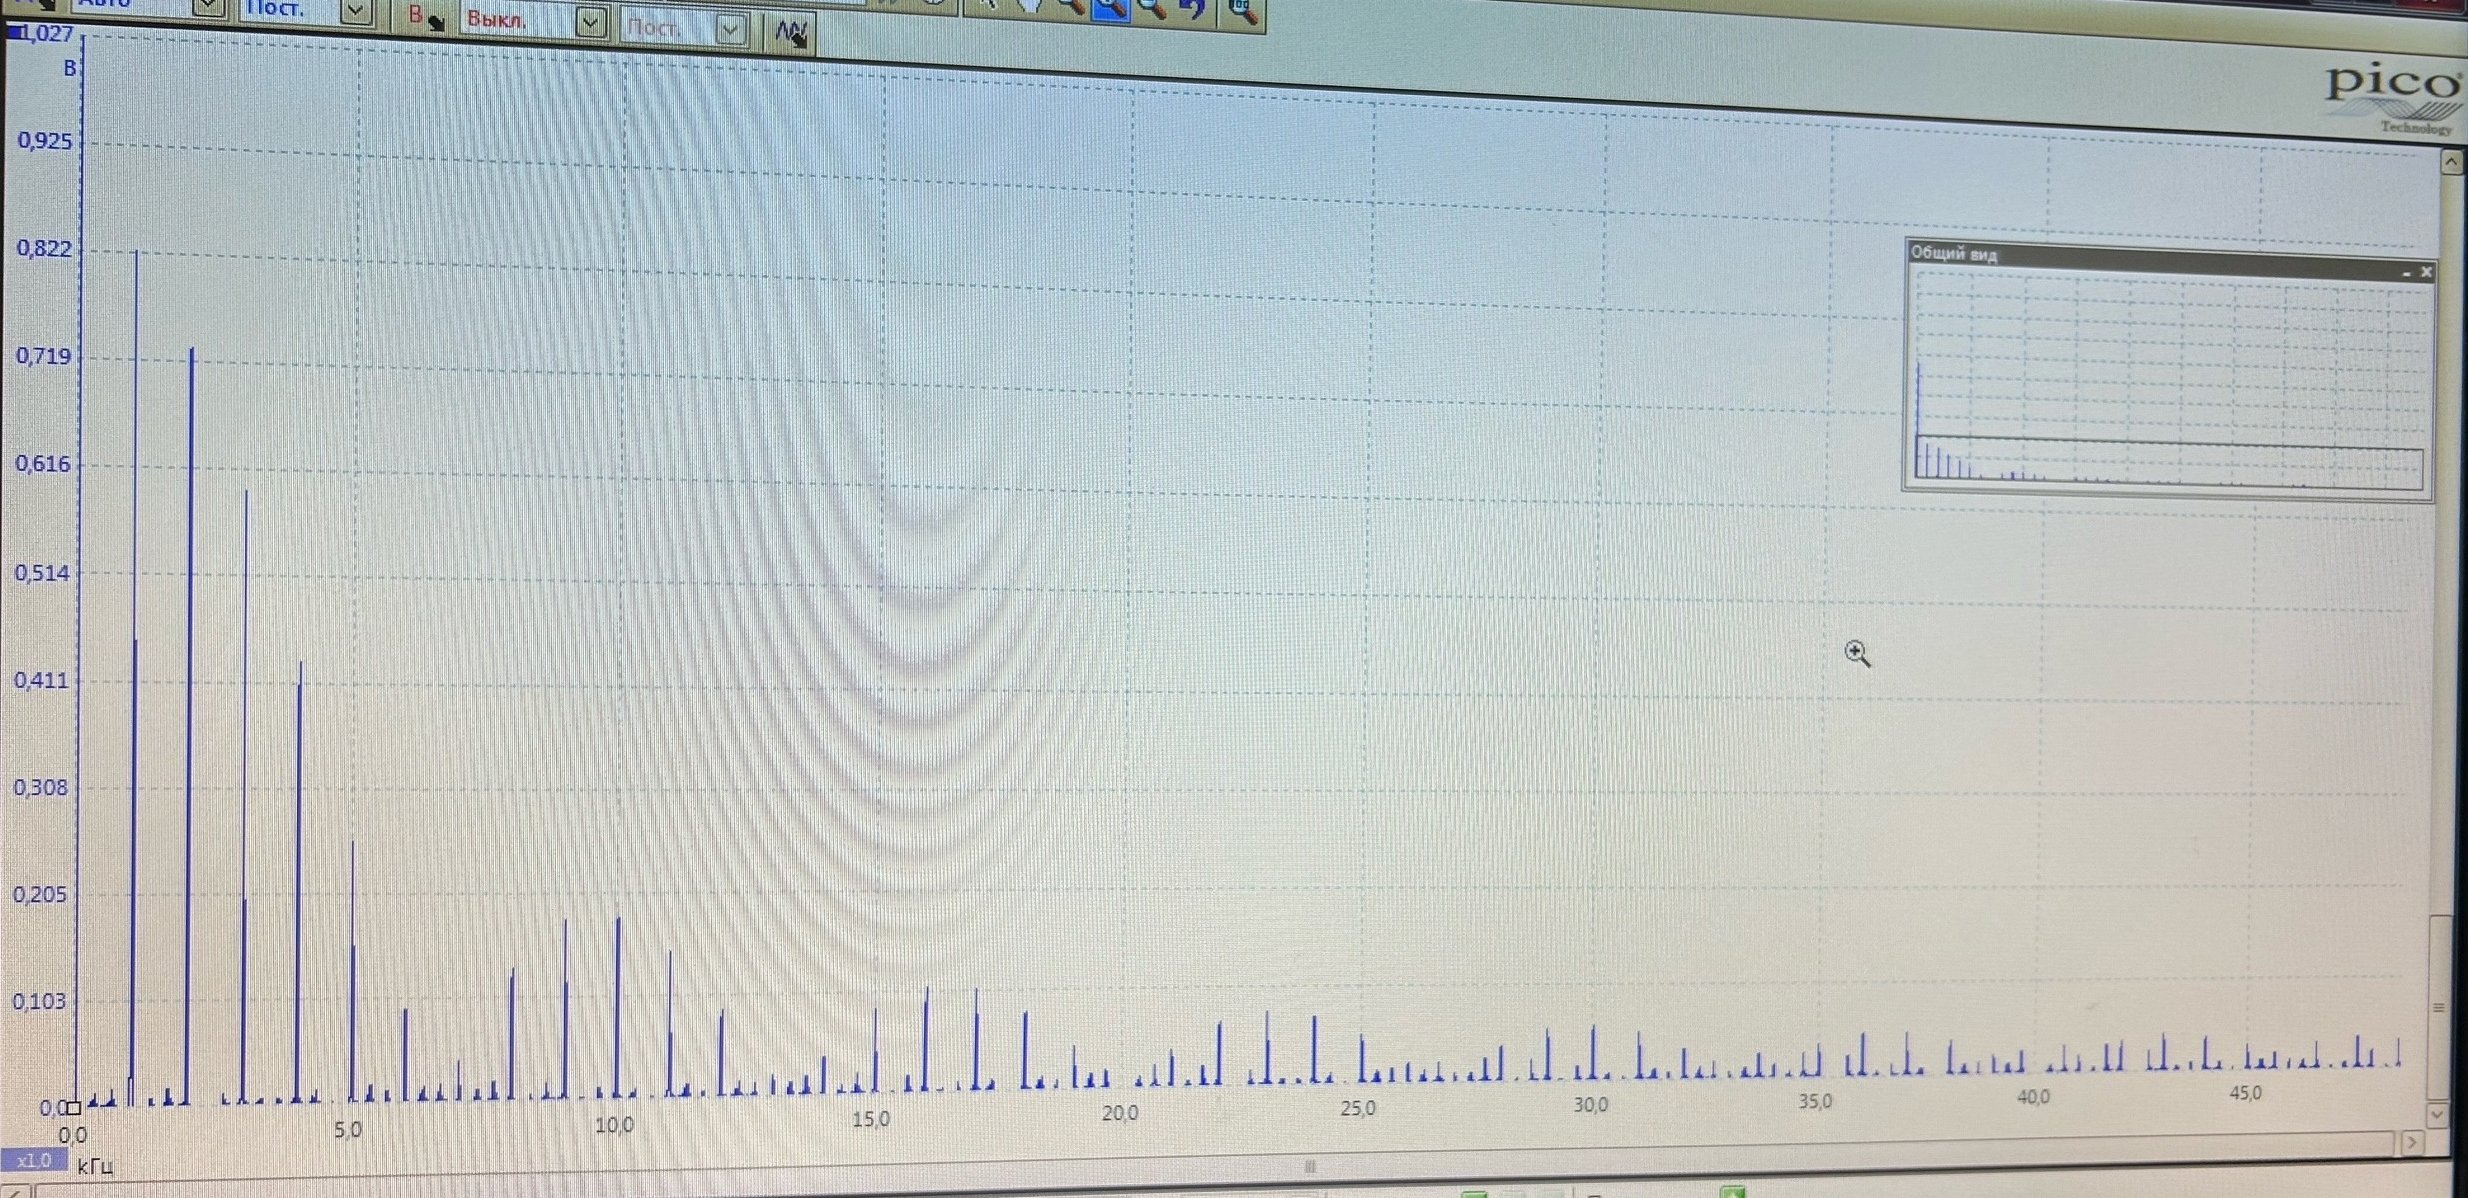
\includegraphics[width=6cm]{./images/nu_1_t_150.jpg}
        \caption{$\nu_{повт} = 1$кГц; $\tau = 150$ мкс}
    \end{subfigure}
    \caption{Изменения спектров при разных параметрах сигнала}
\end{figure}

\begin{table}[h!]
    \centering
    \begin{tabular}{|c|c|c|c|c|c|c|}
        \hline
        $n$ & 1 & 3 & 8 & 9 & 12 & 15\\\hline
        $\nu_n$, кГц & 1 & 3 & 9 & 10 & 12 & 15\\\hline 
        $|a_n|$, усл.ед & 282.6 & 274 & 196.9 & 179.8 & 145.6 & 84.83\\\hline
        $|a_n / a_1|$ эксп & 1 & 0.97 & 0.7 & 0.64 & 0.51 & 0.3\\\hline
        $|a_n / a_1|$ теор & 1 & 0.97 & 0.7 & 0.64 & 0.51 & 0.3\\\hline
    \end{tabular}
    \caption{Сравнение амплитуд и частот гармоник}
\end{table}

\indent Из формулы (1) видно, что полуширина $\Delta \nu$ главного максимума определяется условием $\sin(\omega \tau/2) = 0$ или $\Delta \nu \cdot \tau = 1$. Соотношение $\Delta\nu\cdot\tau \approx 1$ имеет универсальный характер и остается справедливым по порядку величины для произвольного сигнала $f(t)$.

\indentТеперь зафиксируем период повторения $T$ прямоугольного сигнала ($T = 1$ мс; $\nu_{\text{повт}} =$ 1кГц) и будем измерять полную ширину спектра $\Delta \nu$ от центра спектра до гармоники с нулевой амплитудой, изменяя длительность импульса.
\begin{table}[h!]
    \centering
    \begin{tabular}{|c|c|c|c|c|c|c|c|c|c|c|}
        \hline
        $\tau$, мкс & 20& 40& 60& 80& 100& 120& 140& 160& 180& 200\\\hline
        $\Delta\nu$, кГц & 46& 25& 17& 12& 10& 8& 7& 5& 5& 5 \\\hline
    \end{tabular}
    \caption{Зависимость ширины спектра от длительности импульса}
\end{table}

\indentТеперь зафиксируем длительность прямоугольного сигнала $\tau = 50$ мкс и будем менять период повторения $T$, измеряя $\delta \nu$ - расстояния между соседними гармониками.


\begin{table}[h!]
    \centering
    \begin{tabular}{|c|c|c|c|c|c|c|c|c|c|c|c|c|}
        \hline
        $T$, мс & 0.6& 1& 1.4& 1.8& 2.2& 2.6& 3& 3.4& 3.8& 4.2& 4.6& 5 \\\hline
        $\delta\nu$, кГц &1.668& 1.000& 0.723& 0.55& 0.457& 0.383& 0.334& 0.295& 0.264& 0.238& 0.217& 0.200\\\hline
    \end{tabular}
    \caption{Зависимость ширины спектра от длительности импульса}
\end{table}
\indent Из графиков ниже видно, что соотношение неопределенностей выполняется.
\newpage
\begin{figure}[h!]
    \centering
    \begin{subfigure}[b]{0.48\linewidth}
        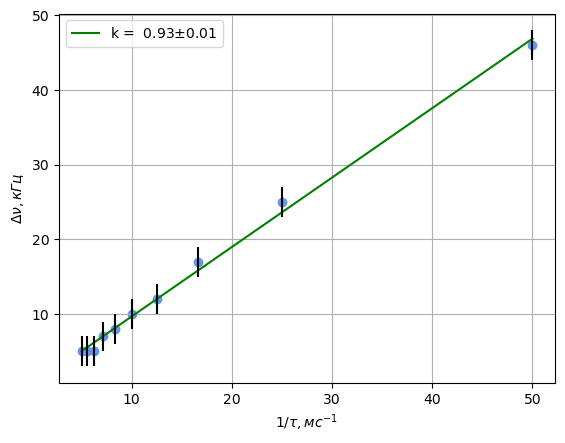
\includegraphics[width=8cm]{plot1.png}
        \caption{График зависимости $\Delta\nu(1 / \tau)$}
    \end{subfigure}
    \hfill
    \begin{subfigure}[b]{0.48\linewidth}
        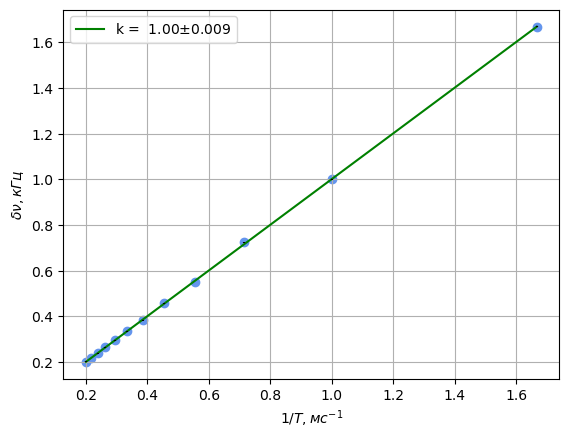
\includegraphics[width=8cm]{plot2.png}
        \caption{График зависимости $\delta\nu(1 /T)$}
    \end{subfigure}
\end{figure}



